% Chapter Template

\chapter{Solution to Log Generation} % Main chapter title

\label{Chapter4} % Change X to a consecutive number; for referencing this chapter elsewhere, use \ref{ChapterX}

\section{Introduction}
In the previous chapters, we have discussed the method to implement the solution to generate a path. Path Generation and Implementation of a method to store the behaviour of the robot with respect to it's neighbours is another issue.
In this chapter, we will cover the method implemented for generation of the log file with respect to the nearby obstacles. 

\section{Constraints}
As we are implementing the solution by following the hypothesis that we wish to see and generate the log in the Digital Twin from the perspective of the God's eye.
We can not use any information that has been published by the robot. Thus, we can not use \textit{scan} topic and sensors to infer data and proceed with data mining.
Therefore, we are only limited to \textit{'use what we can see'}. Odometry describe the position of the robot in the context of the environment. From the god's eye perspective,
we can only see the positional information or \textit{position} of the robot. Therefore, to solve the log generation problem we will only use the \textbf{x} and \textbf{y} positions of the robot.

\section{Using Odometry}
Odometry is a \textit{topic} in ROS which describes the postion of the robot in the coorrdinate system. Odometry message type contains :
\begin{itemize}
    \item \textbf{std\_msgs/Header \textit{header}}, providing a header to the information.
    \item \textbf{string child\_frame\_id}, providing the ID to the frame generated from positional transforms of the robot model.
    \item \textbf{PoseWithCovariance}, describing the linear positional information about the robot i.e the x,y,z position of the robot in the coorrdinate frame.
    \item \textbf{TwistWithCovariance}, describing the angular positional information about the robot i.e the x,y,z angular rotation in the coorrdinate frame.
\end{itemize}

Odometry is the best choice for generation of log file in our implementation. This is because, in our hypothesis, the values should be recorded from the god's eye view (see Figure~\ref{fig:DigitalTwinGodEye}).
Implementation can be done from the robot's LIDAR sensor, although we will get the values from the robot. This implementation will deviate us from our hypothesis. In implementation with the LIDAR sensor, we found out that
the values were not regular. This could be due to incompetency of the LIDAR sensor. We needed to find a different definitive method, using values from odometry. 
In the Figure~\ref{fig:LIDARSensorGrid}, the light grey grid is generated with LIDAR sensor. The process is continous, and not positional. This results in varying discrepency in the data generated. We recorded loss in data, making this approach unusable and further solidifying 
the use of odometry.

\begin{figure}[th]
    \centering
    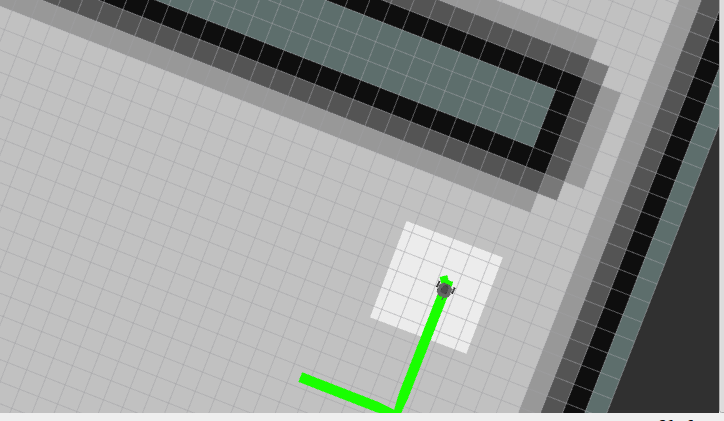
\includegraphics[width=\textwidth]{Figures/local_costmap-grid.png}
    \decoRule
    \caption[]{Grid Generated by Robot}
    \label{fig:LIDARSensorGrid}
\end{figure}

\section{Solution}

\subsection{Obstacle Space}
While generation of the environment in Gazebo, every obstacle is given a position in it. The position of the obstacle is also described by 
using \textbf{x} and \textbf{y} positions of the obstacle. Thus, if we have 44 boxes, we should have 44 different pairs of \textbf{x} and \textbf{y} positions for the obstacle space.
\begin{figure}[th]
    \centering
    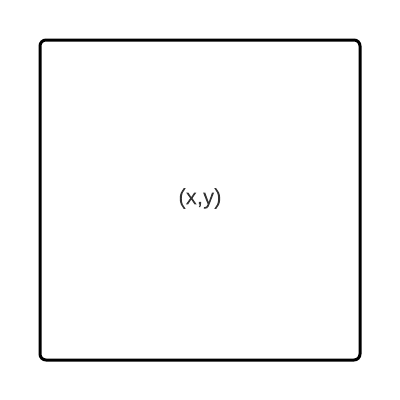
\includegraphics[width=0.3\textwidth]{Figures/simple-obstacle-x-y.png}
    \decoRule
    \caption[]{Obstacle positioning}
    \label{fig:ObstaclePositioning}
\end{figure}

We implemented the log generation algorithm using just 44 different boxes and 44 pairs of \textbf{x} and \textbf{y} positions. We rounded the \textbf{x} and \textbf{y} position to the nearest \textit{point 5}
To generate a 3 by 3 grid, we calculated if the \textbf{x} and \textbf{y} poisitions and adding 0.5 to the values collides with the center of the robot. The method was basic, produced results but was not accurate 
and thus was not suitable for our implementation. We had to increase the number of contact points and change the algorithm, see \ref{finalsol}.

\subsubsection{Correlation of obstacle with robot}
In our digital twin, we wish to use the Odometry positions of the robot as well as the obstacles around the robot. To find if there is an obstacle near the robot, we will have to find a way to correlate the both positions.
A simple algorithm to do so could be,
\begin{itemize}
    \item Finding the x, y position of the robot.
    \item Using the distance of the center of the obstacle with it's borders.
    \item Adding the particular value to the obstacle's position
    \item If it is equal, obstacle is there else not.
    \item Recording this behaviour.
\end{itemize}

The algorithm can be used to produce the obstacle space in a grid around the robot. The algorithm is simple in it's definition but lacks in many use cases.
For example, if the robot just passes around the corner of the obstacle, the algorithm will not be able to show if the position is close to an obstacle or not.
Thus, it needs improvement. 

The improvement should be noted in correlation to the constraints so solve the problem, i.e by only using the position of the robot as well as the obstacle.

\section{Final Solution}\label{finalsol}
In our implementation, the length of the obstacle is 1 unit. Since the obstacle is a square, the length as well as the breadth are 1 unit each.
There is only one position of the obstalcle i.e at the middle (see Figure~\ref{fig:ObstaclePositioning}). We need to improve on the position, and create more pairs of positions where the obstacle is.
We approached this problem by dividing a square into 8 parts with different positional points. The obstacle's distance from the center to an edge is \textbf{0.5 units}.
In order to improve and give more information about the obstacle space to the robot, we had to divide the obstacle into 8 lines with 5 points on each, signifying the coordinates of the obstacle space.
Each of these points are situated at \textbf{0.1 unit} distance from one another. 

\begin{figure}[th]
    \centering
    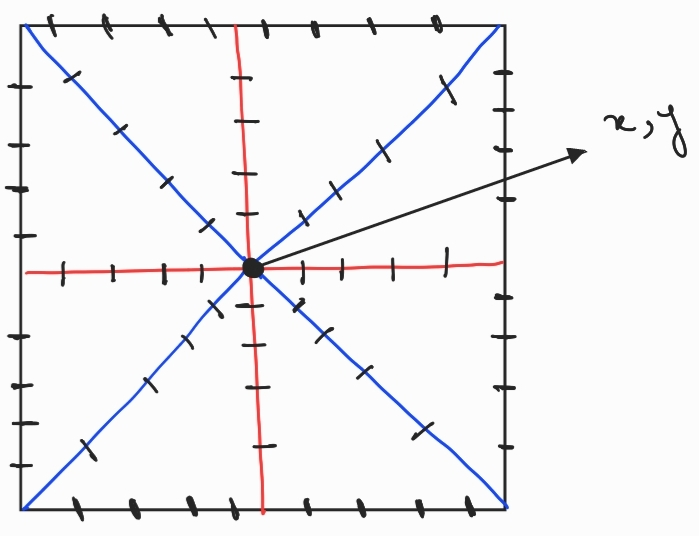
\includegraphics[width=0.4\textwidth]{Figures/improved-obstacle-space.jpg}
    \decoRule
    \caption[]{Divided Obstacle Space}
    \label{fig:ObstacleSpaceDivided}
\end{figure}

As seen in Figure~\ref{fig:ObstacleSpaceDivided}, there are multiple points described in an obstacle space as compared to just one in the previous approach.
Eventhough, we are not using any sensors to get the information, we can name a \textit{perception} range defining the points the robot will check in order to find a point that is present in the obstacle space.
There are 44 obstacles with 72 points each, which means that the obstacle space data structure (python list in our implementation) contains, 3168 pairs of \textbf{x} and \textbf{y} positions.
As the robot will move across the configuration space, the x and y coordinates of the robot will be used to calculate a nearby obsatcle point, if it exists based upon the \textit{perception range} defined in the algorithm.
The obstacle space is saved in a list, and the algorithm will find a point in the perception range of the robot and if it is present in the obstacle space, it will denote it as an obstacle.
Another list will is created, which saves the position values in different grid sizes based upon the perception range of the robot. For example, in a \textit{3 by 3 grid}, the different positions are written to the list, and further to a semi-structured csv file. The log file is then to be used for data mining and reinforcement learning applications.
The log will contain :  

\begin{itemize}
    \item ROS timestamp in seconds.
    \item x and y coordinate of the robot.
    \item the obstacle grid (\textit{any size}) calculated by the algorithm.
    \item x and y coordinates of the goal.
    \item relative x and y coordinates to the goal
    \item manhattan distance of the robot to the goal.
    \item euclidian distance of the robot to the goal.
    \item angular orientation in z axis i.e the rotation of the robot.
\end{itemize}

\section{Conclusion}
